% Chapter Template

\chapter{Conclusiones} % Main chapter title

\label{Chapter5} % Change X to a consecutive number; for referencing this chapter elsewhere, use \ref{ChapterX}


%----------------------------------------------------------------------------------------

%----------------------------------------------------------------------------------------
%	SECTION 1
%----------------------------------------------------------------------------------------

En este capítulo se hace un repaso de las actividades realizadas y se resume la conformidad de los requerimientos del trabajo con respecto a la planificación inicial. También, se hace mención a ciertos puntos a mejorar y a los próximos pasos del proyecto.

\section{Resultados obtenidos}

En general, el proyecto cumplió con todos los requerimientos planteados en la planificación. Se agregaron puntos adicionales, relacionados con la comunicación USB para facilitar el uso del dispositivo, que fueron implementados. Se considera que el objetivo del trabajo se logró de forma satisfactoria: el sistema obtenido facilitó la interacción con los sistemas SN-17 y permite monitorear el estado de los motores en operación.

Se destaca la manifestación de uno de los riesgos especificados en la planificación: el desabastecimiento de componentes electrónicos en el mercado mundial y la dificultad para traerlos a la Argentina generó retrasos en el desarrollo del proyecto e implicó la selección de componentes alternativos. El plan de mitigación de realizar las compras de forma prioritaria fue efectivo y permitió concluir el proyecto a tiempo.

Para el correcto desarrollo del trabajo, se utilizaron los conocimientos adquiridos a lo largo del posgrado, en particular:

\begin{itemize}
	\item Programación de microprocesadores: funcionamiento general de un microcontrolador, programación de periféricos (comunicación y timers) y máquinas de estado.
	\item Ingeniería de software: construcción de la arquitectura del software en capas, utilización de repositorios y definición de los servicios requeridos de cada uno de los drivers implementados.
	\item Protocolos de comunicación en sistemas embebidos: Utilización de diversos protocolos dentro del sistema, entre ellos, CAN, UART, SPI e I2C.
	\item Arquitectura de microprocesadores: Utilización de optimizaciones de compilador, cambios en linker script para almacenaje en memoria no volátil de información.
	\item Testing de software en sistemas embebidos: uso de herramientas de pruebas automáticas para encontrar errores en el software desarrollado.
	\item Diseño de circuitos impresos: recomendaciones para el desarrollo físico de la plaqueta. Utilización de reglas para desarrollo de PCB. Esquemáticos eléctricos separados por subcircuitos.
	\item Diseño para manufacturabilidad: selección de componentes para facilitar el ensamble, técnicas de soldadura recomendadas y consideraciones para ensamble automático.
\end{itemize}

Es importante notar que el sistema pudo ser montado y probado en una línea de montaje real en desarrollo en la planta industrial de Cambre ICyFSA. Los resultados de los ensayos realizados fueron satisfactorios.

%En la figura \ref{fig:au-0037} se muestra una imagen de la línea de ensamblaje en cuestión y se puede visualizar el sistema desarrollado junto con los actuadores que cuentan con los sistemas SN-17.
%
%\begin{figure}[htbp]
%	\centering
%	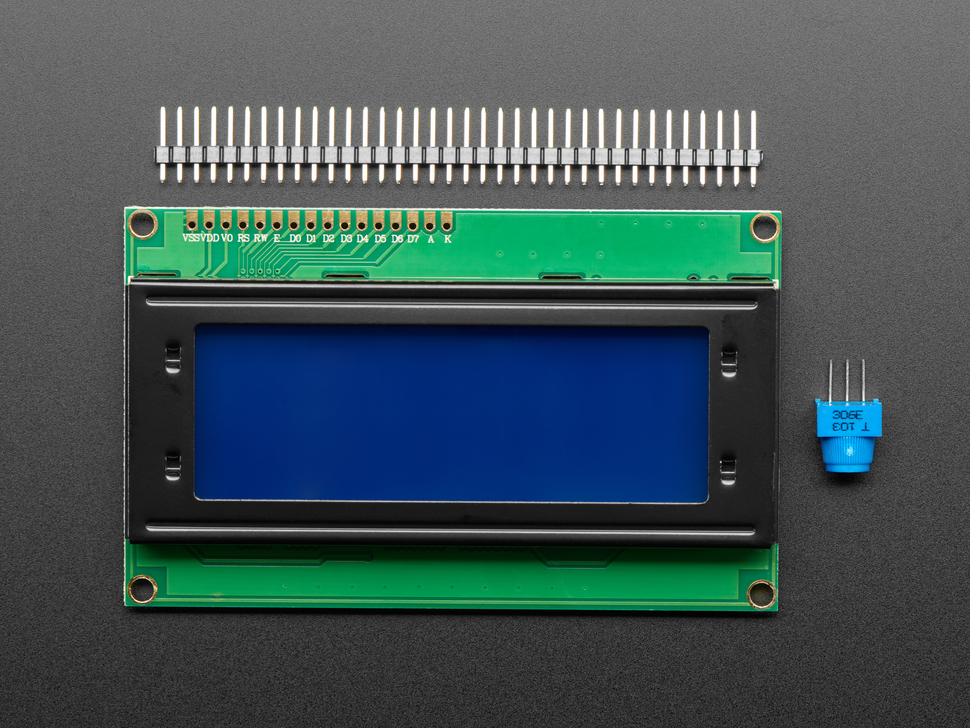
\includegraphics[scale=1]{./Figures/LCD.jpg}
%	\caption{Línea de ensamble automática con SCI-CAN - ARAMR FIGURA}
%	\label{fig:au-0037}
%\end{figure}

%----------------------------------------------------------------------------------------
%	SECTION 2
%----------------------------------------------------------------------------------------
\section{Próximos pasos}

Con el dispositivo implementado en las líneas productivas de Cambre ICyFSA, se le hará un seguimiento exhaustivo para corregir posibles errores y realizar posibles mejoras que puedan surgir con el uso del dispositivo. 

Se plantea como trabajo futuro:
\begin{itemize}
	\item Modificar el firmware para que trabaje con un sistema operativo, en lugar de \textit{bare metal}.
	\item Generar una interfaz gráfica para PC utilizando la conexión USB implementada.
	\item Implementar mensajes CAN entre diferentes dispositivos SN-17, sin la interacción del SCI-CAN para generar movimientos coordinados.
	\item Generar identificación dinámica de dispositivos, sin necesidad de utilizar identificadores de CAN fijos.
	\item Implementar otros protocolos de comunicación industriales, permitiendo más diversidad de interacciones.
\end{itemize}
